\documentclass[11pt]{article}
\usepackage[unicode]{hyperref}
\usepackage[utf8]{inputenc}
\usepackage[a4paper,total={17cm,24cm},left=2cm,top=3cm]{geometry}
\usepackage{xcolor}
\usepackage[IL2]{fontenc}
\usepackage{times}
\usepackage[czech]{babel}
\usepackage{multirow}
\usepackage[ruled, linesnumbered, noline, czech, longend]{algorithm2e}
\usepackage{graphicx} 
\usepackage{pdflscape}


\begin{document}

\begin{titlepage}

\begin{center}

\textsc{ \Huge Vysoké učení technické v~Brně\\}

\textsc{\huge Fakulta informačních technologií\\}

 
\vspace{\stretch{0.382}}
{\LARGE Typografie a publikování – 3. projekt \\ }
{\Huge Tabulky a obrázky \\}
\vspace{\stretch{0.618}}
\end{center}
{\large \today \hfill Eduard Frlička (xfrlic00)}
\end{titlepage}


\section{Úvodní strana}
Název práce umístěte do zlatého řezu a nezapomeňte uvést dnešní datum a vaše jméno a příjmení.

\section{Tabulky}
Pro sázení tabulek můžeme použít buď prostředí \ \texttt{tabbing} \ nebo prostředí \ \texttt{tabular}.

\subsection{Prostředí \ \texttt{tabbing}}
Při použití \ \texttt{tabbing} \ vypadá tabulka následovně:

% \begin{table}[h]
%     \begin{tabbing}{lllll}
%     Ovoce         & Cena  & Množství &  &  \\
%     Jablka        & 25,90 & 3 kg     &  &  \\
%     Hrušky        & 27,40 & 2,5 kg   &  &  \\
%     Vodní melouny & 35,-  & 1 ks     &  & 
%     \end{tabbing}
% \end{table}



\begin{tabbing}
    \hspace{2.75cm}     \= \hspace{1.25cm}   \= \hspace{1.25cm}     \kill
    \textbf{Ovoce} \> \textbf{Cena} \> \textbf{Množství} \\
    Jablka \> 25,90 \> 3 kg \\
    Hrušky \> 27,40 \> 2,5 kg\\
    Vodní melouny \> 35,- \> 1 ks\\
\end{tabbing}



\noindent
Toto prostředí se dá také použít pro sázení algoritmů, ovšem vhodnější je použít 
prostředí \ \texttt{algorithm} \ nebo \ \texttt{algorithm2e} \ (viz sekce \ref{Algoritmy}).


\subsection{Prostředí \ \texttt{tabular}}
Další možností, jak vytvořit tabulku, je použít prostředí \ \texttt{tabular}. Tabulky pak 
budou vypadat takto
\footnote{Kdyby byl problem s cline, zkuste se podívat třeba sem: http://www.abclinuxu.cz/tex/poradna/show/325037}
:

\begin{table}[h!]
    \centering
    \catcode`\-=12
    \begin{tabular}{|c|c|c|}
    \cline{1-3}
    {\multirow{2}{*}{\textbf{Měna}}}                     & \multicolumn{2}{c|}{\textbf{Cena}}                                             \\ \cline{2-3}
                                                & \textbf{nákup}                             & \textbf{prodej}                            \\ \cline{1-3}
    EUR                                         & 25,227                            &  26,943                            \\
    GBP                                         & 29,368                            &  31,492                          \\
    USD                                         & 21,260                            &  22,661                       \\ \cline{1-3}
    \end{tabular}
    \caption{Tabulka kurzů k dnešnímu dni}
    \label{Tab1}
\end{table}

\begin{table}[h!]
    \centering
    \catcode`\-=12
    \begin{tabular}{|c|c|}
    \cline{1-2}
        $A$ & $\neg A$ \\ \cline{1-2}
        \textbf{P} & N \\ \cline{1-2}
        \textbf{O} & O \\ \cline{1-2}
        \textbf{X} & X \\ \cline{1-2}
        \textbf{N} & P \\ \cline{1-2}
    \end{tabular}
    \begin{tabular}{|c|c|c|c|c|c|}
        \hline
        \multicolumn{2}{|c|}{\multirow{2}{*}{{$A \wedge B$}}} & \multicolumn{4}{c|}{B}                            \\ \cline{3-6} 
        \multicolumn{2}{|c|}{}                              & \textbf{P} & \textbf{O} & \textbf{X} & \textbf{N} \\ \hline
        \multirow{4}{*}{A}           & \textbf{P}           & P          & O          & X          & N          \\ \cline{2-6} 
                                     & \textbf{O}           & O          & O          & N          & N          \\ \cline{2-6} 
                                     & \textbf{X}           & X          & N          & X          & N          \\ \cline{2-6} 
                                     & \textbf{N}           & N          & N          & N          & N          \\ \hline
    \end{tabular}
    \begin{tabular}{|c|c|c|c|c|c|}
        \hline
        \multicolumn{2}{|c|}{\multirow{2}{*}{$A \vee B$}} & \multicolumn{4}{c|}{B}                            \\ \cline{3-6} 
        \multicolumn{2}{|c|}{}                      & \textbf{P} & \textbf{O} & \textbf{X} & \textbf{N} \\ \hline
        \multirow{4}{*}{A}       & \textbf{P}       & P          & P          & P          & P          \\ \cline{2-6} 
                                    & \textbf{O}       & P          & O          & P          & O          \\ \cline{2-6} 
                                    & \textbf{X}       & P          & P          & X          & X          \\ \cline{2-6} 
                                    & \textbf{N}       & P          & O          & X          & N          \\ \hline
    \end{tabular}
    \begin{tabular}{|c|c|c|c|c|c|}
        \hline
        \multicolumn{2}{|c|}{\multirow{2}{*}{$A \rightarrow B$}} & \multicolumn{4}{c|}{B}                            \\ \cline{3-6} 
        \multicolumn{2}{|c|}{}                      & \textbf{P} & \textbf{O} & \textbf{X} & \textbf{N} \\ \hline
        \multirow{4}{*}{A}       & \textbf{P}       & P          & O          & X          & N          \\ \cline{2-6} 
                                    & \textbf{O}       & P          & O          & P          & O          \\ \cline{2-6} 
                                    & \textbf{X}       & P          & P          & X          & X          \\ \cline{2-6} 
                                    & \textbf{N}       & P          & P          & P          & P          \\ \hline
    \end{tabular}
    \caption{Protože Kleeneho trojhodnotová logika už je \uv{zastaralá}, uvádíme si zde příklad čtyřhodnotové logiky}
    \label{Tab2}
\end{table}




\newpage
\section{Algoritmy}
\label{Algoritmy}
Pokud budeme chtít vysázet algoritmus, můžeme použít prostředí \ \texttt{algorithm\footnotemark} \ nebo 
\footnotetext{Pro nápovědu, jak zacházet s prostředím algorithm, můžeme zkusit tuhle stránku: \\
http://ftp.cstug.cz/pub/tex/CTAN/macros/latex/contrib/algorithms/algorithms.pdf.}
{algorithm2e\footnotemark}.
Příklad použití prostředí \ \texttt{algorithm2e} \ viz Algoritmus \ref{alg}.
\footnotetext{Pro algorithm2e zase tuhle:
http://ftp.cstug.cz/pub/tex/CTAN/macros/latex/contrib/algorithm2e/algorithm2e.pdf.}


\IncMargin{2em}
\begin{algorithm}
    \SetNlSty{Large}{}{:}
    \SetAlgoNoLine

    \Indm
    \Indm
    \KwIn{$\left(X_{t-1}, u_{t}, z_{t}\right)$}
    \KwOut{$X_{t}$ }
    \Indp
    \Indp

    \BlankLine

    $\overline{X_{t}}=X_{t}=0$ \\
    \For{$k=1$ \normalfont to $M$}{
        $x_{t}^{[k]}=$ \emph{sample\_motion\_model}$(u_{t}, x_{t-1}^{[k]})$ \\
        $\omega_{t}^{[k]}=$ \emph{measurement\_model} $(z_{t}, x_{t}^{[k]}, m_{t-1})$ \\
        $m_{t}^{[k]}= updated\_occupancy\_grid (z_{t}, x_{t}^{[k]}, m_{t-1}^{[k]})$ \\
        $\overline{X_{t}}=\overline{X_{t}}+\langle x_{x}^{[m]}, \omega_{t}^{[m]}\rangle$ \\
    }
    \For{$k=1$ \normalfont to $M$}{
        draw $i$ with probability $\approx \omega_{t}^{[i]}$\\
        add $\langle x_{x}^{[k]}, m_{t}^{[k]}\rangle$ to $X_{t}$ \\
    }
    \KwRet{$X_{t}$}
        \caption{\textsc{FastSLAM}}
    \label{alg}
  \end{algorithm}


\section{Obrázky}
Do našich článků můžeme samozřejmě vkládat obrázky. Pokud je obrázkem fotografie,
můžeme klidně použít bitmapový soubor. Pokud by to ale mělo být nějaké schéma nebo
něco podobného, je dobrým zvykem takovýto obrázek vytvořit vektorově.



\begin{figure}[h]
    \centering
    \scalebox{0.4}{
        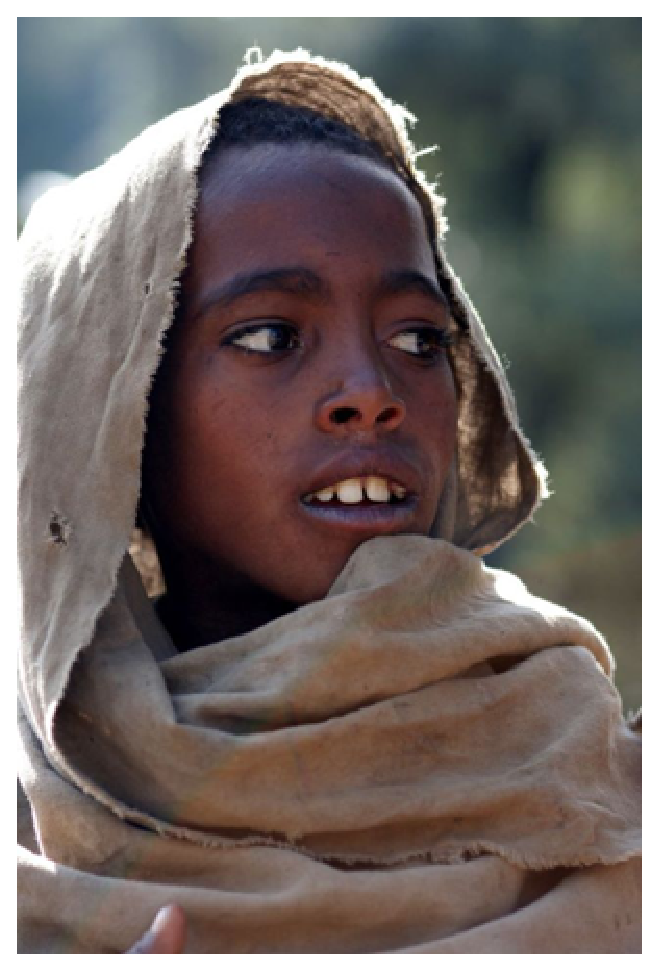
\includegraphics{etiopan.eps}
        \reflectbox{
            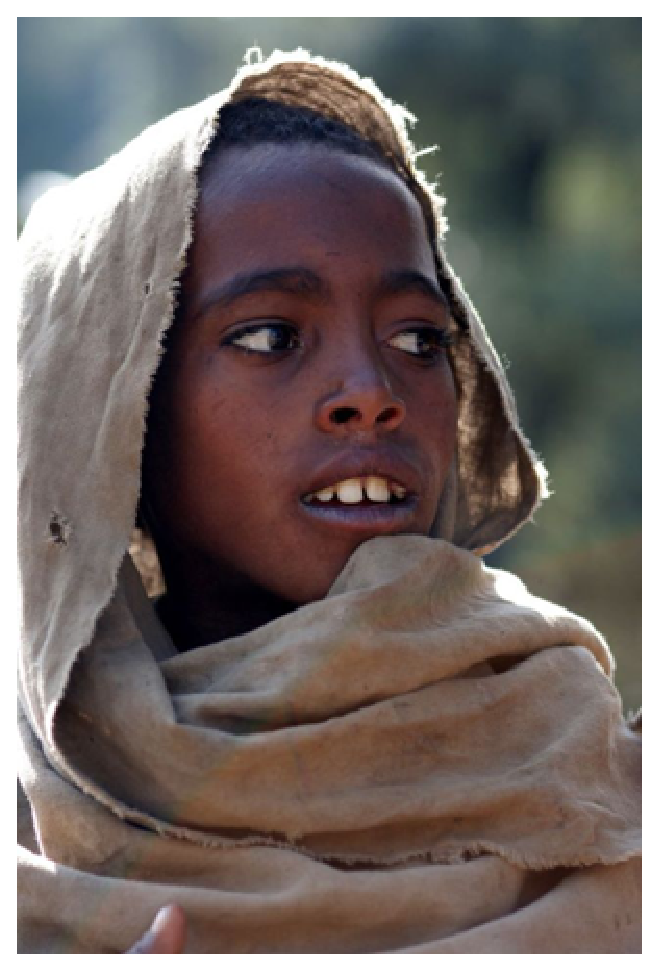
\includegraphics{etiopan.eps}
            }
            }
            \caption{ Malý Etiopánek a jeho bratříček}
    \label{Obr1}
\end{figure}


\newpage
Rozdíl mezi vektorovým . . .
\begin{figure}[h]
    \centering
    \scalebox{0.4}{
        
\includegraphics{oniisan.eps}
        }
        \caption{ Vektorový obrázek }
        \label{Obr2}
    \end{figure}
    
\noindent
. . . a bitmapovým obrázkem

\begin{figure}[h]
    \centering
    \scalebox{0.6}{
        
\includegraphics{oniisan2.eps}
        }
        \caption{ Bitmapový obrázek }
    \label{Obr3}
\end{figure}

\noindent
se projeví například při zvětšení.

Odkazy (nejen ty) na obrázky \ref{Obr1}, \ref{Obr2} a \ref{Obr3}, na  
tabulky \ref{Tab1} a \ref{Tab2} a také na algoritmus \ref{alg} jsou udělány pomocí 
křížových odkazů. Pak je ovšem potřeba zdrojový soubor přeložit dvakrát.

Vektorové obrázky lze vytvořit i přímo v \LaTeX u, například pomocí prostředí 
\ \texttt{picture}.

\newpage
\begin{landscape}
    \begin{figure}[h]
        \bigskip \bigskip
        \centering
        \fbox{
        \begin{picture}(500,300)(0,0)      
            %plot
            \put(20,20){\line(1,0){460}}
            \put(20,50){\line(1,0){5}}
            \put(475,50){\line(1,0){5}}
            \multiput(25,20)(10,0){46}{\line(0,1){40}}
            \multiput(25,60)(20,0){23}{\line(1,0){10}}
            \multiput(35,50)(20,0){22}{\line(1,0){10}}
            
            %obrys
            \put(30,100){\line(1,0){440}}
            
            \put(30,100){\line(0,1){70}}
            \put(30,170){\line(1,0){120}}
            
            \put(470,170){\line(-1,0){120}}
            \put(470,100){\line(0,1){70}}
            
            \put(150,220){\line(1,0){200}}
            \put(150,100){\line(0,1){120}}
            \put(350,100){\line(0,1){120}}
            
            %strecha
            \put(30,170){\line(1,1){30}}
            \put(60,200){\line(1,0){90}}
            
            \put(470,170){\line(-1,1){30}}
            \put(440,200){\line(-1,0){90}}
            
            \put(150,220){\line(1,1){40}}
            \put(350,220){\line(-1,1){40}}
            \put(190,260){\line(1,0){120}}
            
            %dvere
            \multiput(230,100)(20,0){3}{\line(0,1){50}}
            \put(230,150){\line(1,0){40}}
            
            %okna-vlavo
            \put(45,120){\framebox(20,30){}}
            \put(45,130){\line(1,0){20}}
            \put(45,140){\line(1,0){20}}
            \put(55,120){\line(0,1){30}}
            
            \put(80,120){\framebox(20,30){}}
            \put(80,130){\line(1,0){20}}
            \put(80,140){\line(1,0){20}}
            \put(90,120){\line(0,1){30}}
            
            \put(115,120){\framebox(20,30){}}
            \put(115,130){\line(1,0){20}}
            \put(115,140){\line(1,0){20}}
            \put(125,120){\line(0,1){30}}
            
            %okna-stred
            \put(180,120){\framebox(20,30){}} 
            \put(180,130){\line(1,0){20}} 
            \put(180,140){\line(1,0){20}}
            \put(190,120){\line(0,1){30}}
            
            \put(300,120){\framebox(20,30){}}
            \put(300,130){\line(1,0){20}}
            \put(300,140){\line(1,0){20}}
            \put(310,120){\line(0,1){30}}
            %--------
            \put(180,170){\framebox(20,30){}}
            \put(180,180){\line(1,0){20}}
            \put(180,190){\line(1,0){20}}
            \put(190,170){\line(0,1){30}}
            
            \put(220,170){\framebox(20,30){}}
            \put(220,180){\line(1,0){20}}
            \put(220,190){\line(1,0){20}}
            \put(230,170){\line(0,1){30}}
            
            \put(260,170){\framebox(20,30){}}
            \put(260,180){\line(1,0){20}}
            \put(260,190){\line(1,0){20}}
            \put(270,170){\line(0,1){30}}
            
            \put(300,170){\framebox(20,30){}}
            \put(300,180){\line(1,0){20}}
            \put(300,190){\line(1,0){20}}
            \put(310,170){\line(0,1){30}}
            
            
            %okna-vpravo
            \put(365,120){\framebox(20,30){}}
            \put(365,130){\line(1,0){20}}
            \put(365,140){\line(1,0){20}}
            \put(375,120){\line(0,1){30}}
            
            \put(400,120){\framebox(20,30){}}
            \put(400,130){\line(1,0){20}}
            \put(400,140){\line(1,0){20}}
            \put(410,120){\line(0,1){30}}
            
            \put(435,120){\framebox(20,30){}}
            \put(435,130){\line(1,0){20}}
            \put(435,140){\line(1,0){20}}
            \put(445,120){\line(0,1){30}}
            
            %slnko
            \put(50,270){\circle{40}}
            
        \end{picture}}
        \caption{Vektorový obrázek středné školy, do které jsem chodil}
        \label{fig:4}
    \end{figure}
    \end{landscape}
    

\end{document}